%%%%%%%%%%%%%%%%%%%%%%%%%%%%%%%%%%%%%%%%%%%%%%%%%%%%%%%%%%%%%%%%%%%%%%%%%%%%%%%%
%%            _   _            __   ____                                      %%
%%           / / | |          / _| |  __|                                     %%
%%           | |_| |  _   _  / /   | |_                                       %%
%%           |  _  | | | | | | |   |  _|                                      %%
%%           | | | | | |_| | \ \_  | |__                                      %%
%%           |_| |_| \_____|  \__| |____| microLab                            %%
%%                                                                            %%
%%           Bern University of Applied Sciences (BFH)                        %%
%%           Quellgasse 21                                                    %%
%%           Room HG 4.33                                                     %%
%%           2501 Biel/Bienne                                                 %%
%%           Switzerland                                                      %%
%%                                                                            %%
%%           http://www.microlab.ch                                           %%
%%%%%%%%%%%%%%%%%%%%%%%%%%%%%%%%%%%%%%%%%%%%%%%%%%%%%%%%%%%%%%%%%%%%%%%%%%%%%%%%
\chapter{{\sc GECKO4com} IO}
\label{appen:4com}
This appendix describes the different IO components and the connection diagrams.
\section{VGA screen and message windows}
Figure~\ref{fig:vga screenshot} show the VGA screen produced by the {\sc GECKO4com}. In
Figure~\ref{fig:vga screenshot} the three different text screens are marked in brown.
\begin{figure}[h]
\centering%
\includegraphics[width=\columnwidth]{figs/vga_screens}
\caption{The VGA screen as produced by the {\sc GECKO4com}. The different
message windows are marked in brown.}
\label{fig:vga screenshot}
\end{figure}
\section{Buttons, switch and LEDs}
Figure~\ref{fig:but sw leds} shows the {\sc GECKO4com}'s part of the {\sc GECKO4main}. The
different buttons, the switch and the bicolor LEDs are marked.
\begin{figure}[h]
\centering%
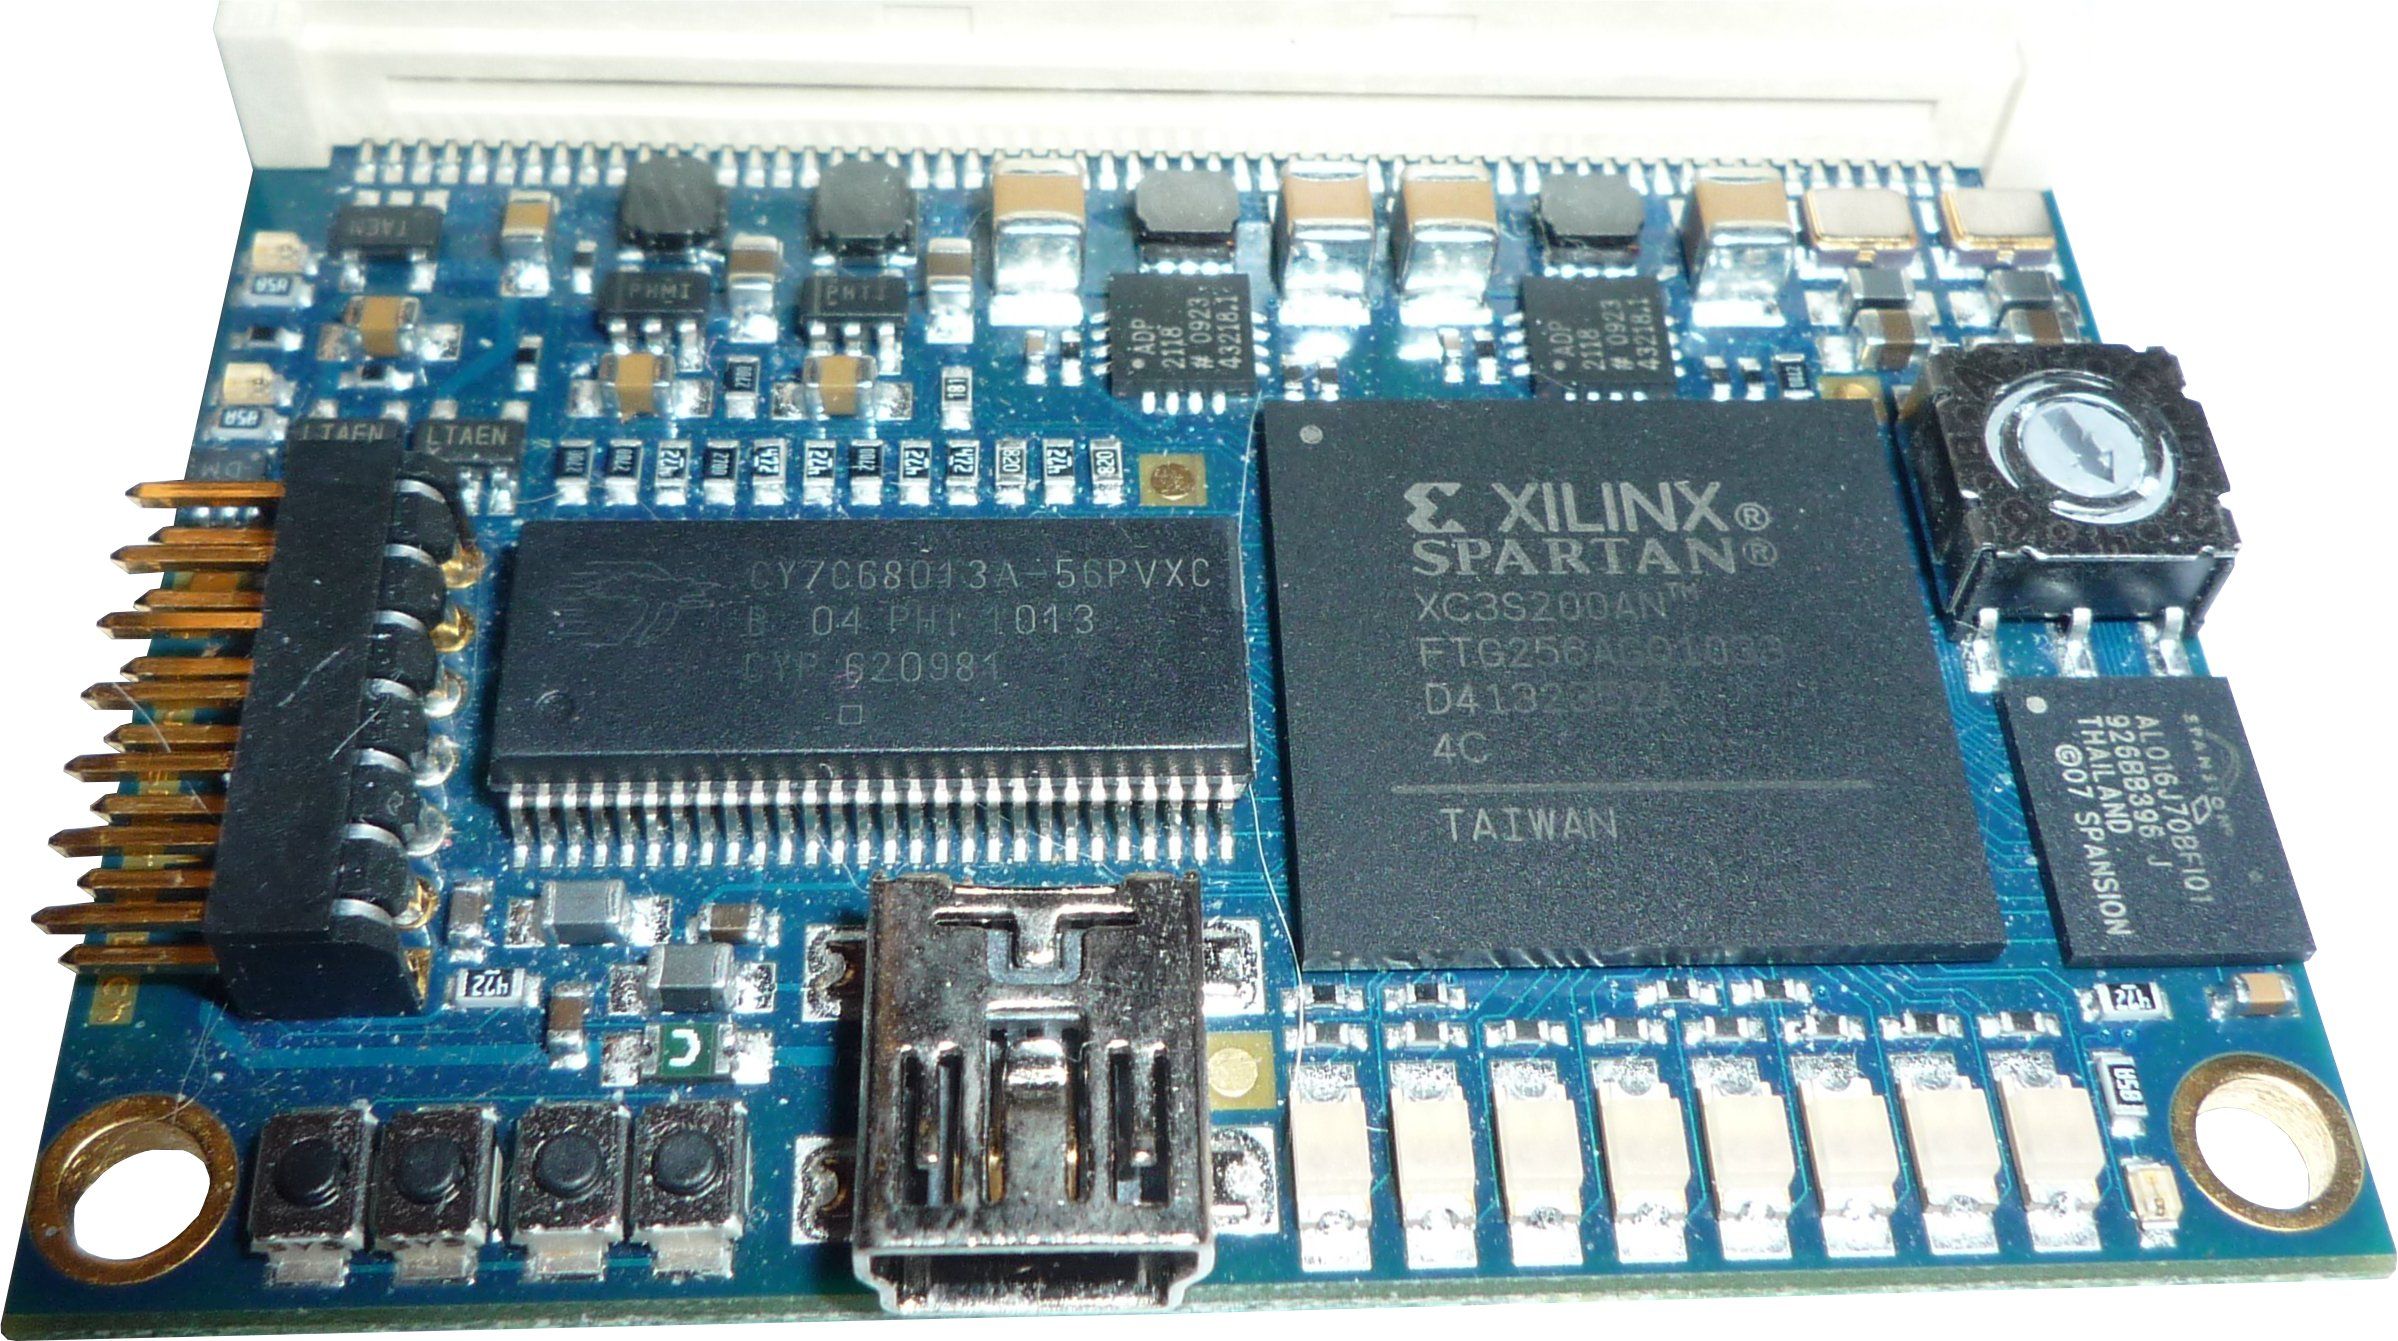
\includegraphics[width=\columnwidth]{figs/gecko4com}
\caption{The buttons, the switch and the LEDs of the {\sc GECKO4com}.}
\label{fig:but sw leds}
\end{figure}
\newpage
\section{VGA connection and RS232}
The bottom of Figure~\ref{fig:but sw leds} shows the {\sc GECKO4main}'s dual function connector and
its pin numbering.
This connector can be used to connect a VGA-screen and a
RS232 connector. Table~\ref{tab: conn vga rs232} lists the pin-numbers of this connector, the
corresponding signal names and their connection on a female VGA connector,
respectively their connections on a female RS232 connector. All signals not
listed in Table~\ref{tab: conn vga rs232} should be left unconnected.\\
\textit{Note: The 3.3V power supply can be used to supply level translators for
the RS232 communication (for example the MAX232).\note}
\begin{table}[h]
\centering%
\begin{tabular}{|c|l|c|}
\hline
\textbf{Dual function pin}&\textbf{Signal name}&\textbf{VGA pin}\\
\hline
\hline
\verb+1+&Ground&\verb+5,10+\\
\hline
\verb+3+&Vertical Sync&\verb+14+\\
\hline
\verb+4+&Horizontal Sync&\verb+13+\\
\hline
\verb+10+&Blue&\verb+3+\\
\hline
\verb+12+&Green&\verb+2+\\
\hline
\verb+13+&Analog Ground&\verb+6,7,8+\\
\hline
\verb+14+&Red&\verb+1+\\
\hline
\hline
\textbf{Dual function pin}&\textbf{Signal name}&\textbf{RS232 pin}\\
\hline
\hline
\verb+2+&\multicolumn{2}{c|}{3.3V power supply}\\
\hline
\verb+7+&RS232 RxD&\verb+3+\\
\hline
\verb+9+&RS232 TxD&\verb+2+\\
\hline
\verb+11+&Ground&\verb+5+\\
\hline
\end{tabular}
\caption{Connection diagram of the dual function connector to a VGA connector
and a RS232 connector (9-pol. Zero Modem connection)}
\label{tab: conn vga rs232}
\end{table}
